\documentclass{beamer}
\usepackage[T1]{fontenc}
\usepackage[utf8]{inputenc}

\usetheme{Madrid}
\usecolortheme{default}
\usepackage{amsmath,amssymb,amsfonts,amsthm}
\usepackage{txfonts}
\usepackage{tkz-euclide}
\usepackage{listings}
\usepackage{adjustbox}
\usepackage{array}
\usepackage{tabularx}
\usepackage{gvv}
\usepackage{lmodern}
\usepackage{gensymb}
\usepackage{circuitikz}
\usepackage{tikz}
\usepackage{graphicx}
\usepackage{capt-of}
\usepackage{multicol}

\setbeamertemplate{page number in head/foot}[totalframenumber]

\usepackage{tcolorbox}
\tcbuselibrary{minted,breakable,xparse,skins}

\definecolor{bg}{gray}{0.95}
\DeclareTCBListing{mintedbox}{O{}m!O{}}{%
  breakable=true,
  listing engine=minted,
  listing only,
  minted language=#2,
  minted style=default,
  minted options={%
    linenos,
    gobble=0,
    breaklines=true,
    breakafter=,,
    fontsize=\small,
    numbersep=8pt,
    #1},
  boxsep=0pt,
  left skip=0pt,
  right skip=0pt,
  left=25pt,
  right=0pt,
  top=3pt,
  bottom=3pt,
  arc=5pt,
  leftrule=0pt,
  rightrule=0pt,
  bottomrule=2pt,
  toprule=2pt,
  colback=bg,
  colframe=orange!70,
  enhanced,
  overlay={%
    \begin{tcbclipinterior}
    \fill[orange!20!white] (frame.south west) rectangle ([xshift=20pt]frame.north west);
    \end{tcbclipinterior}},
  #3,
}
\lstset{
    language=C,
    basicstyle=\ttfamily\small,
    keywordstyle=\color{blue},
    stringstyle=\color{orange},
    commentstyle=\color{green!60!black},
    numbers=left,
    numberstyle=\tiny\color{gray},
    breaklines=true,
    showstringspaces=false,
}

\title{2.10.39}
\subtitle{Vector Geometry}
\author{EE25BTECH11010 - Arsh Dhoke}
\date{}

\begin{document}

\begin{frame}
\titlepage
\end{frame}

\begin{frame}{Question}
Let $\vec{a}=2\vec{i}+\vec{j}+\vec{k}$,\quad
$\vec{b}=\vec{i}+2\vec{j}-\vec{k}$ and a unit vector $\vec{c}$ be coplanar.  
If $\vec{c}$ is perpendicular to $\vec{a}$, then $\vec{c}=$

\begin{multicols}{2}
\begin{enumerate}
\item \( \tfrac{1}{\sqrt{2}}(-\vec{j}+\vec{k})\) 
\item \( \tfrac{1}{\sqrt{3}}(-\vec{i}-\vec{j}-\vec{k})\) 
\item \( \tfrac{1}{\sqrt{5}}(\vec{i}-2\vec{j})\) 
\item \( \tfrac{1}{\sqrt{3}}(\vec{i}-\vec{j}-\vec{k})\) 
\end{enumerate}
\end{multicols}
\end{frame}

\begin{frame}{Solution}
\begin{tabular}{|c|c|}
\hline
\textbf{Name} & \textbf{Value} \\
\hline
Circle & $\vec{x}^\top\vec{x} - a^2 = 0$ \\
\hline
Line & $\vec{x} = \myvec{\tfrac{a}{\sqrt{2}} \\ 0} + \kappa\myvec{0 \\ 1}$ \\
\hline
\end{tabular}


\begin{align}
\vec{c}&=\vec{a}+k\vec{b} \\
\vec{c}&=\myvec{2+k\\1+2k\\1-k} \\
\vec{a}^T\vec{c}&=0 \\
2(2+k)+1(1+2k)+1(1-k)&=0 \\
6+3k&=0 
\end{align}
\end{frame}

\begin{frame}{Solution (continued)}
\begin{align}
k&=-2 \\
\vec{c}&=\myvec{0\\-3\\3} \\
\|\vec{c}\| &=\sqrt{0^2+(-3)^2+3^2}=3\sqrt{2} \\
\vec{c}&=\frac{1}{3\sqrt{2}}\myvec{0\\-3\\3} \\
\vec{c}&=\frac{1}{\sqrt{2}}\myvec{0\\-1\\1}
\end{align}
\textbf{Thus, option 1 is correct.}
\end{frame}

\begin{frame}{Graph}
\begin{figure}
\centering
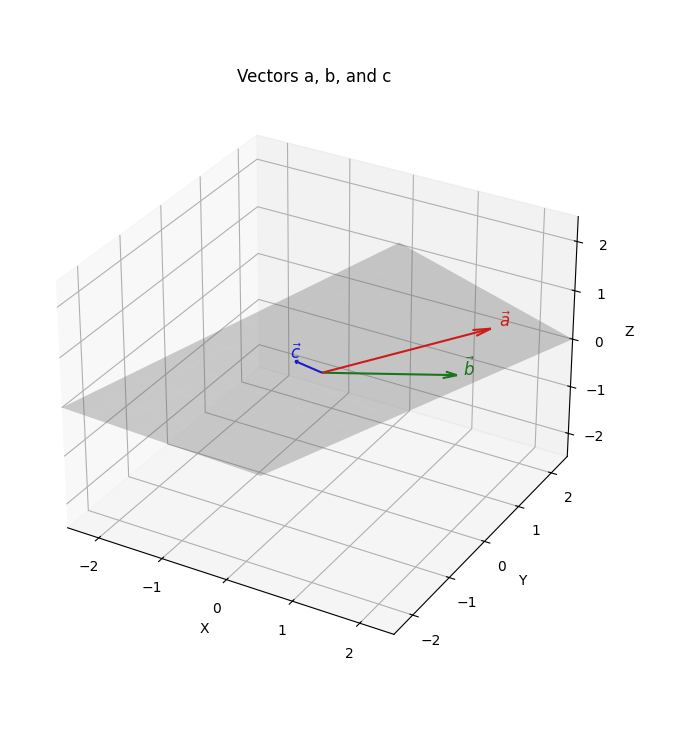
\includegraphics[height=0.8\textheight, keepaspectratio]{figs/q5.png}
\caption{Graph of vectors}
\end{figure}
\end{frame}

\begin{frame}[fragile]
    \frametitle{C Code}
\begin{lstlisting}
#include <math.h>

typedef struct {
    double x;
    double y;
    double z;
} Vec3;

Vec3 find_unit_vector_c(void) {
    double a[3] = {2, 1, 1};
    double b[3] = {1, 2, -1};

    double dot_ab = a[0]*b[0] + a[1]*b[1] + a[2]*b[2];
    double dot_aa = a[0]*a[0] + a[1]*a[1] + a[2]*a[2];
    double k = - (double)dot_aa / dot_ab;

    double x = a[0] + k*b[0];
    double y = a[1] + k*b[1];
    

\end{lstlisting}
\end{frame}

\begin{frame}[fragile]
    \frametitle{C Code}
\begin{lstlisting}
    double z = a[2] + k*b[2];
    double mag = sqrt(x*x + y*y + z*z);

    Vec3 result;
    result.x = x / mag;
    result.y = y / mag;
    result.z = z / mag;

    return result;
}
\end{lstlisting}
\end{frame}

\begin{frame}[fragile]
    \frametitle{Python Code}
\begin{lstlisting}
import numpy as np
import matplotlib.pyplot as plt
from mpl_toolkits.mplot3d import Axes3D

# Define vectors
a = np.array([2, 1, 1])
b = np.array([1, 2, -1])
c = np.array([0, -1, 1]) / np.sqrt(2)  # unit vector

# Compute normal to plane (a x b)
n = np.cross(a, b)
A, B, C = n  # plane coefficients
# Plane equation: A*x + B*y + C*z = 0 (through origin)

# Create a grid for x and y
x_vals = np.linspace(-2.5, 2.5, 10)
y_vals = np.linspace(-2.5, 2.5, 10)
X, Y = np.meshgrid(x_vals, y_vals)
\end{lstlisting}
\end{frame}

\begin{frame}[fragile]
    \frametitle{Python Code}
\begin{lstlisting}
# Solve for Z from plane equation (avoid divide by zero)
Z = (-A * X - B * Y) / C

# Create 3D figure
fig = plt.figure(figsize=(9, 9))
ax = fig.add_subplot(111, projection='3d')

origin = np.zeros(3)

# Plot the plane as a translucent surface
ax.plot_surface(X, Y, Z, alpha=0.3, color='gray')

# Plot vectors
ax.quiver(*origin, *a, color='r', arrow_length_ratio=0.1)
ax.quiver(*origin, *b, color='g', arrow_length_ratio=0.1)
ax.quiver(*origin, *c, color='b', arrow_length_ratio=0.1)
\end{lstlisting}
\end{frame}

\begin{frame}[fragile]
    \frametitle{Python Code}
\begin{lstlisting}
# Add text labels near arrowheads
ax.text(*(a * 1.05), r'$\vec{a}$', color='r', fontsize=12)
ax.text(*(b * 1.05), r'$\vec{b}$', color='g', fontsize=12)
ax.text(*(c * 1.2),  r'$\vec{c}$', color='b', fontsize=12)

# Set axes limits and labels
ax.set_xlim([-2.5, 2.5])
ax.set_ylim([-2.5, 2.5])
ax.set_zlim([-2.5, 2.5])
ax.set_xlabel('X')
ax.set_ylabel('Y')
ax.set_zlabel('Z')

ax.grid(True)
plt.title("Vectors a, b, and c")
plt.savefig("/home/arsh-dhoke/ee1030-2025/ee25btech11010/matgeo/2.10.39/figs/q5.png")
plt.show()

\end{lstlisting}
\end{frame}

\begin{frame}[fragile]
    \frametitle{Python+ C Code}
\begin{lstlisting}
import ctypes
import numpy as np
import matplotlib.pyplot as plt
from mpl_toolkits.mplot3d import Axes3D  # needed for 3D plotting

# --- Mirror the C struct ---
class Vec3(ctypes.Structure):
    _fields_ = [("x", ctypes.c_double),
                ("y", ctypes.c_double),
                ("z", ctypes.c_double)]

# --- Load the shared library ---
lib = ctypes.CDLL("./code.so")
lib.find_unit_vector_c.restype = Vec3  # C returns a Vec3 struct

# --- Call the C function ---
result = lib.find_unit_vector_c()
unit_vector = np.array([result.x, result.y, result.z])
\end{lstlisting}
\end{frame}

\begin{frame}[fragile]
    \frametitle{Python+ C Code}
\begin{lstlisting}
print("Unit vector from C:", unit_vector)

# --- Plot the unit vector ---
fig = plt.figure(figsize=(6,6))
ax = fig.add_subplot(111, projection='3d')

# Draw axes
ax.quiver(0, 0, 0, unit_vector[0], unit_vector[1], unit_vector[2],
          color='blue', arrow_length_ratio=0.1, linewidth=2)

# Mark the tip of the vector
ax.scatter(unit_vector[0], unit_vector[1], unit_vector[2],
           color='red', s=50, label='Unit Vector')

# Label axes
ax.set_xlim([0,1]); ax.set_ylim([0,1]); ax.set_zlim([0,1])
ax.set_xlabel('X')
\end{lstlisting}
\end{frame}


\begin{frame}[fragile]
    \frametitle{Python+ C Code}
\begin{lstlisting}
ax.set_ylabel('Y')
ax.set_zlabel('Z')
ax.set_title('Unit Vector from C Library')
ax.legend()

plt.tight_layout()
plt.savefig("/home/arsh-dhoke/ee1030-2025/ee25btech11010/matgeo/2.10.39/figs/q5.png")
plt.show()

\end{lstlisting}
\end{frame}

\end{document}